\begin{figure}[htbp]
\section*{ CYP21A2}
\centering
\begin{subfigure}[b]{0.95\textwidth}
\centering
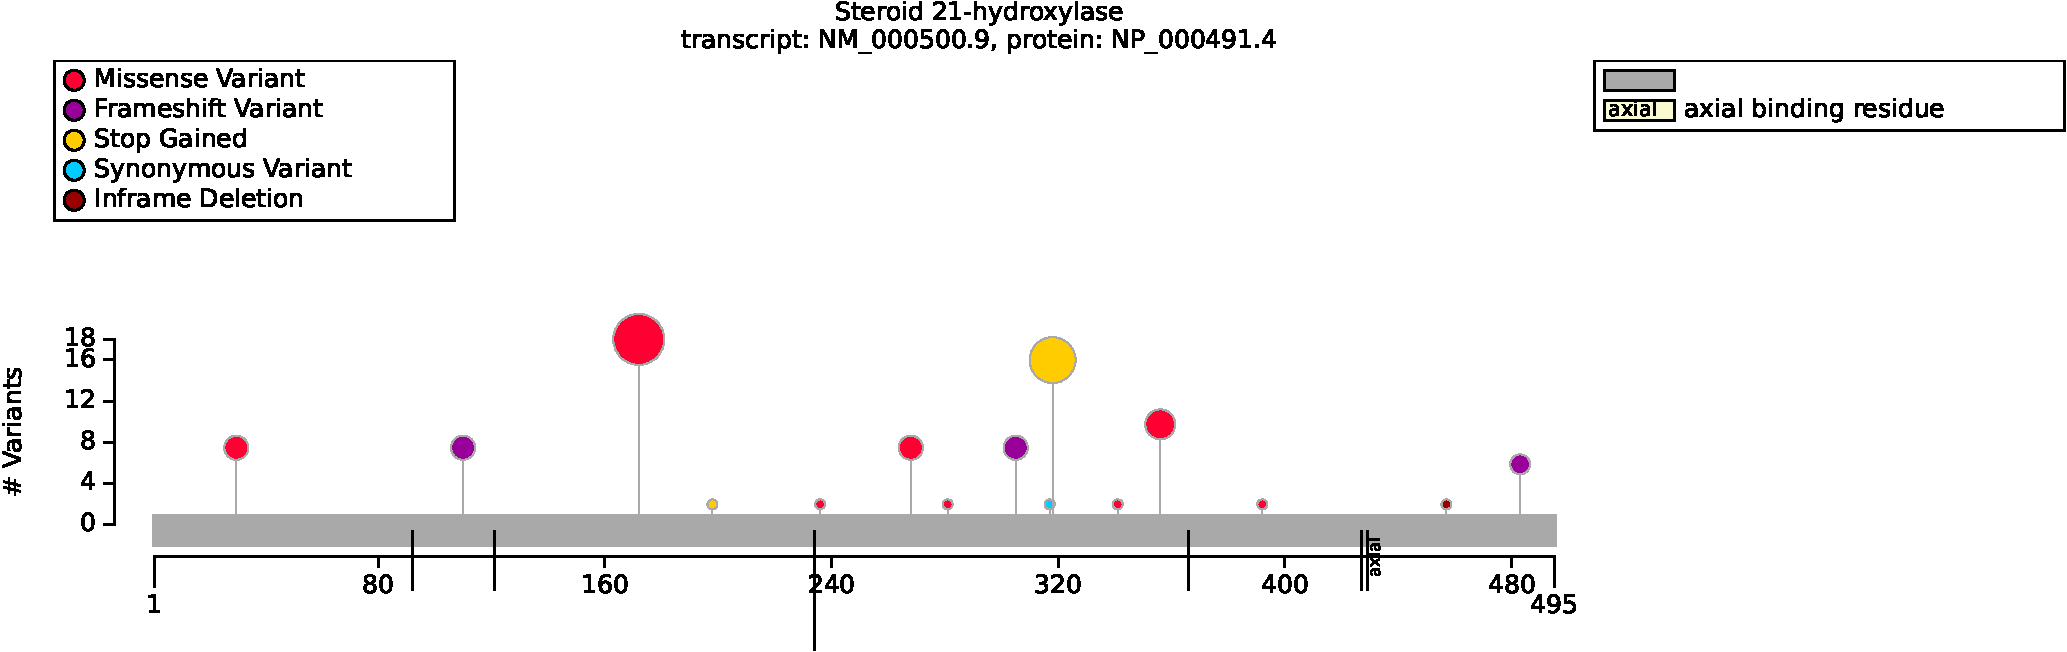
\includegraphics[width=\textwidth]{ img/CYP21A2_protein_diagram.pdf} 
\captionsetup{justification=raggedright,singlelinecheck=false}
\caption{Distribution of variants in CYP21A2}
\end{subfigure}

\vspace{2em}

\begin{subfigure}[b]{0.95\textwidth}
\centering
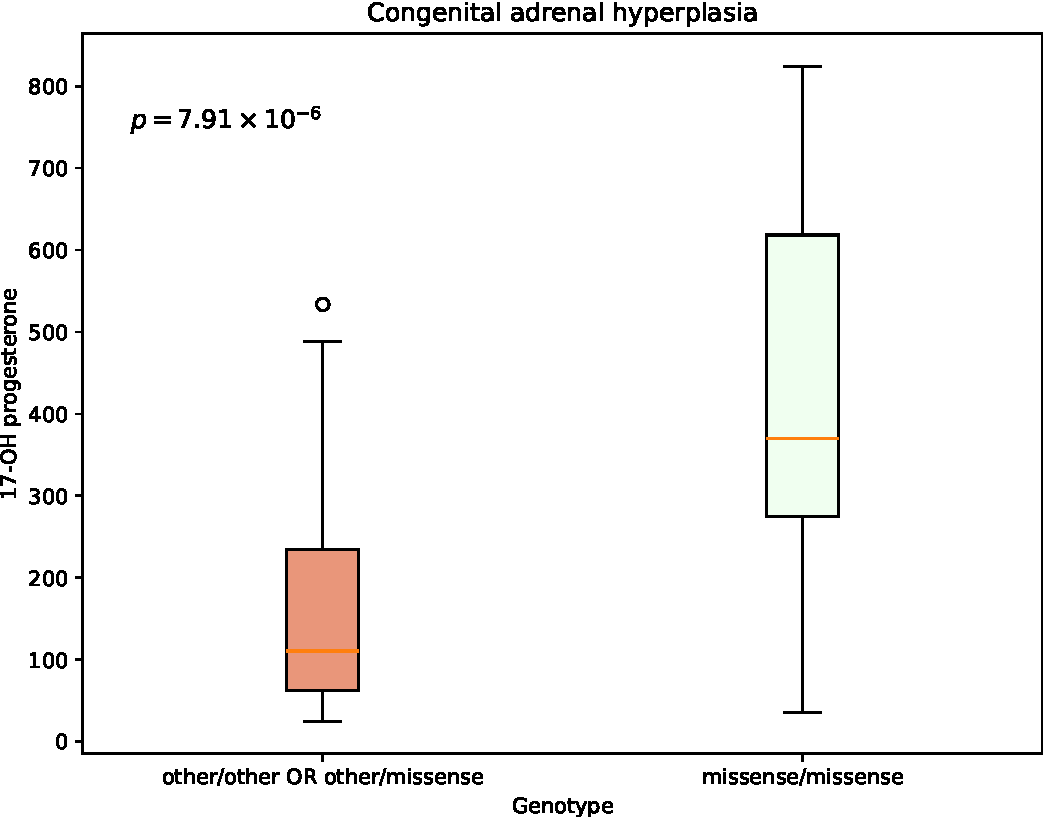
\includegraphics[width=0.3\textwidth]{ img/CYP21A2_stats.pdf} 
\captionsetup{justification=raggedright,singlelinecheck=false}
\caption{t-test. 17-hydroxyprogesterone level. CYP21A2 missense variants are compared with other variants.}
\end{subfigure}

\vspace{2em}

\begin{subfigure}[b]{0.95\textwidth}
\captionsetup{justification=raggedright,singlelinecheck=false}
\resizebox{\textwidth}{!}{
\begin{tabular}{llllrr}
\toprule
Description & Variable & Genotype (A) & Genotype (B) & p-value & xrefs\\
\midrule
17-Hydroxyprogesterone [Mass/volume] in Serum or Plasma [LOINC:1668-3] & LOINC:1668-3 & other/other OR other/missense & missense/missense & $7.91\times 10^{-6}$ & \cite{PMID_30968594}\\
\bottomrule
\end{tabular}
}
\caption{t-test to compare other/other OR other/missense and missense/missense with respect to LOINC:1668-3. }
\end{subfigure}

\vspace{2em}

\caption{ The cohort comprised 69 individuals (34 females, 35 males). A total of 27 HPO terms were used to annotate the cohort. 
Disease diagnosis: Adrenal hyperplasia, congenital, due to 21-hydroxylase deficiency (OMIM:201910).
It is assumed that the mildest mutation determines the phenotype in compound heterozygotes. Several missense variants display the highest residual activities.
High levels of 17-hydroxyprogesterone may be observed with  21-hydroxylase deficiency \cite{PMID_30968594}.
A total of 122 unique variant alleles were found in \textit{CYP21A2} (transcript: \texttt{NM\_000500.9}, protein id: \texttt{NP\_000491.4}).}
\end{figure}
